%!TEX root = ../paper.tex

\section{Pulsarcast}
\label{section:pulsarcast}

Pulsarcast is a peer to peer, pub-sub, topic-based system focused on
reliability, eventual delivery guarantees, and data persistence. Properties
usually associated with centralised pub-sub solutions. 

We opted for the more straightforward topic-based subscription model given
that, in our view, a well structured and implemented topic-based model is more
than enough for a significant percentage of our use cases. In the end, we
compromise a bit of the expressiveness of the system in order to avoid bringing
more complexity in, something we believe will pay off.

Pulsarcast is a fully decentralised solution, which means that each node plays
a crucial part in fulfilling the system's purpose, delivering events and
ensuring their dissemination. Conceptually speaking, Pulsarcast provides four
methods for clients and applications to interact with the system, \emph{create}
a topic, \emph{subscribe} to a topic, \emph{unsubscribe} from a topic and
\emph{publish} an event in a topic. From a broader perspective, Pulsarcast
relies on two overlays to fulfil its needs. Kadmelia DHT, used for peer
discovery, content discovery and to bootstrap our other overlay, our per-topic
dissemination trees. These trees are critical for us to disseminate information
across our decentralised network.

When a peer publishes an event or creates a new topic a set of the overlays
previously described is used accordingly. For Pulsarcast, both of these
actions, happen to take a similar course. That is because the system views
these pieces of information (or descriptors as we call it) as fairly similar,
given their importance.

Every topic and event is stored in the Kadmelia DHT before being forwarded
through the topic dissemination trees. This ensures the data is persisted by a
set of nodes (that might even be extraneous to the topic at hand) and anyone is
later able to fetch the data using only the DHT if they want to. Once
persisted, we forward the data through the appropriate dissemination trees
previously built. On the other hand, when someone wants to fetch a piece of
data (a topic or an event) it starts by performing a local search in the
system, it might have been something that the node has run through when
forwarding events across their dissemination trees. If this fails, though, a
query to the DHT is in order.

Pulsarcast has a set of two fundamental data structures to which we refer to as
\textbf{event} and \textbf{topic descriptors}. All of our data structures are
immutable, content addressable and linked together to form a Directed Acyclic
Graph (Merkle DAG). Events link both to their respective topic descriptor and a
past event in that topic. Topics, on the other hand, link to their sub-topics
(if any) and a previous version of themselves. Figure \ref{fig:pulsarcast-dag}
provides a broader picture of how it all fits together. Immutability and
content-addressability give us verifiability. Consequently, the assurance that
the state of our distributed system is the same no matter where we are
accessing it from or who is viewing it. It also allows us to build a notion of
history which plays nicely into a pub-sub scenario. Through these links and the
mechanisms described so far, users and applications are free to rebuild their
topic and event history to any point they wish. Be that because they were not
part of the network at the time or because they missed out due to some system
or network failure, acting as a NACK (not acknowledged) for relevant events.
This is the core of Pulsarcast's eventual delivery guarantees.

\begin{figure}[hb!]
  \centering
  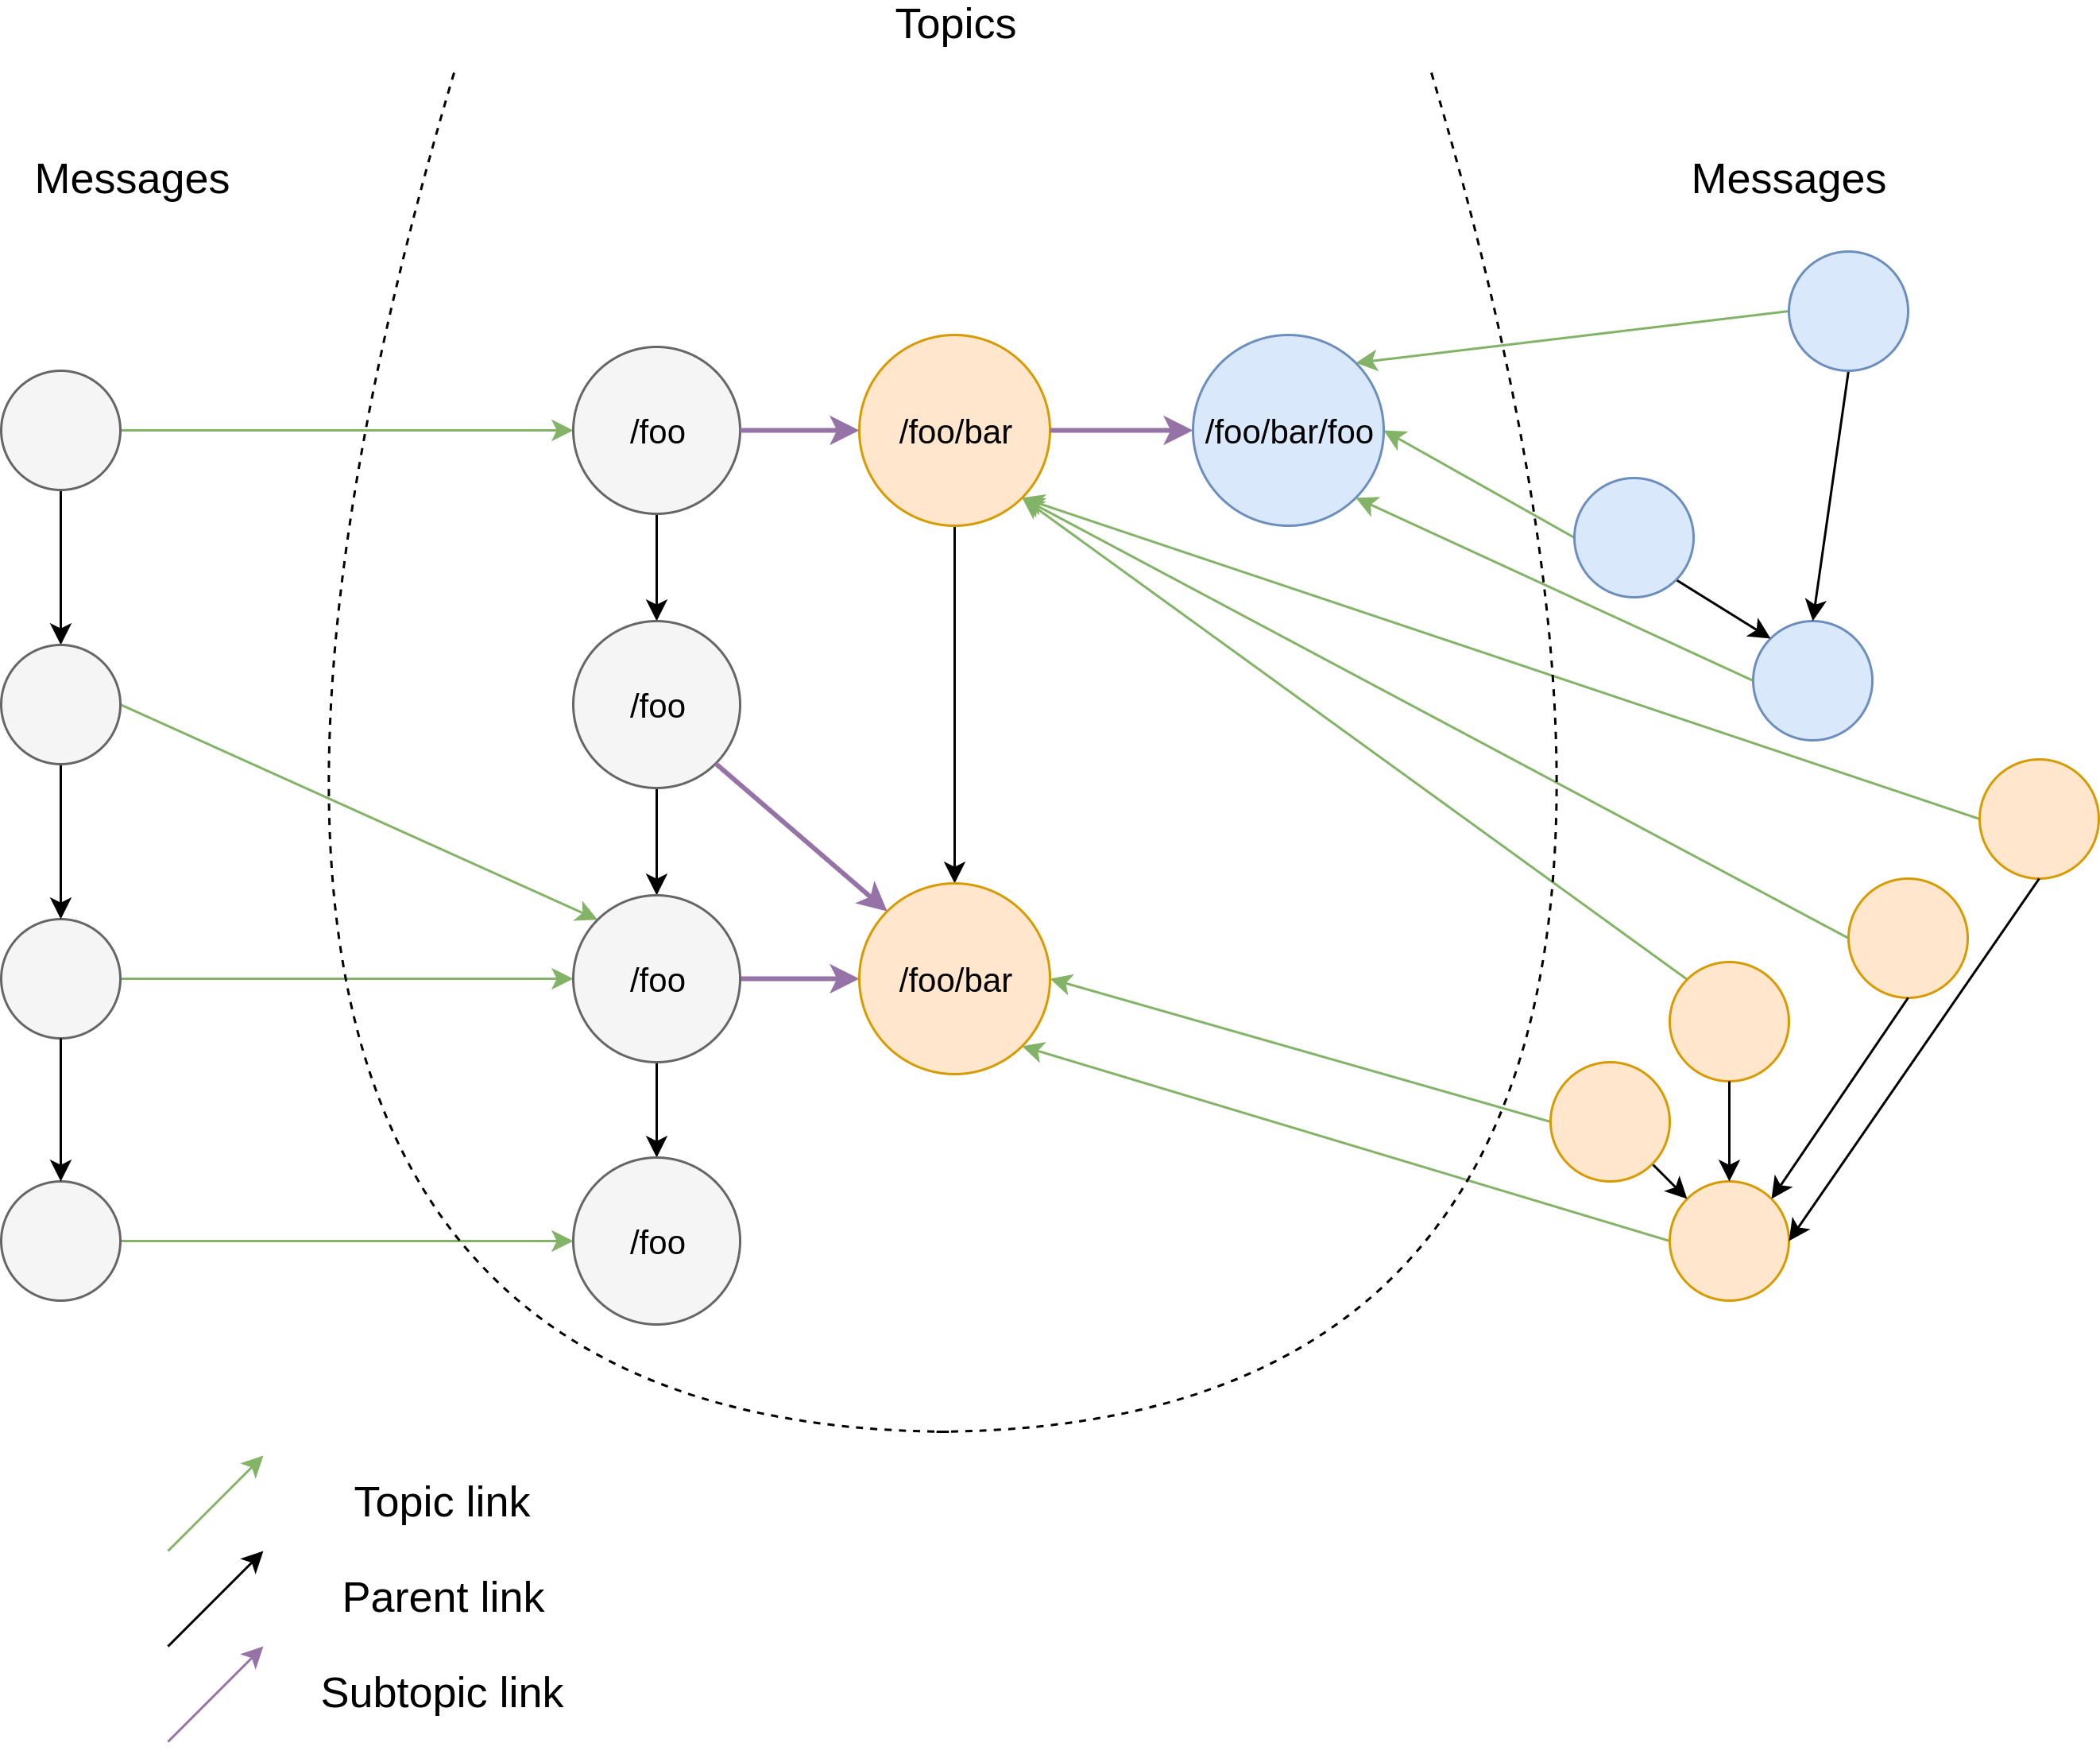
\includegraphics[width=0.45\textwidth]{img/pulsarcast-dag.png}
  \caption{Representation of the Pulsarcast DAG}
  \label{fig:pulsarcast-dag}
\end{figure}

Given we are discussing addressability and linking between content, the
representation used for our identifiers is an important part of our system
specification. That was one of the main reasons for us to borrow inspiration
from systems like IPFS and decided to use \emph{CIDs} (Content
Identifiers)~\footnote{\url{https://github.com/multiformats/cid}}.  A CID is a
self-describing content-addressed identifier. It uses cryptographic hashes to
achieve content addressing and is powered by
\emph{multihash}~\footnote{\url{https://github.com/multiformats/multihash}}.
Multihash is a convention for representing the output of many different
cryptographic hash functions in a compact, deterministic encoding that is
accommodating of future change. This is because multihash encodes the type of
hash function used to produce the output. All of the relevant identifiers in
our system are CIDs. This includes node identifiers as well as the identifiers
for both event descriptors and topic descriptors themselves (given they are the
hash of its content). The descriptors contain a set of relevant metadata as
well as the actual information that they refer to. The following JSON like
Listings \ref{topic-descriptor} and \ref{event-descriptor} provide an accurate
description of the schema and format of our data structures. We will cover some
of the properties.

% \noindent\begin{minipage}{\textwidth}
% \vspace{8pt}
\begin{lstlisting}[float, language=JSON,caption={Topic descriptor schema in a JSON based format},label={topic-descriptor}]
{
  "name": <string>,
  "author": <peer-id>,
  "parent": {                     //The parent link for this topic
    "/": <topic-id>
  },
  "#": {                          //Sub topic links
		"meta": {												//Meta topic
			"/": "zdpuAkx9dPaPve3H9ezrtSipCSUhBCGt53EENDv8PrfZNmRnk"
		},
    <topic-name>: {
      "/": <topic-id>
    },
    ...
  },
  "metadata": {
    "created": <date-iso-8601>,
    "protocolVersion": <string>,  //Pulsarcast protocol version
    "allowedPublishers": {        //If enabled, whitelist of allowed publishers
      "enabled": <boolean>,
      "peers": [ <peer-id> ]
    },
    "requestToPublish": {         //Enable request to publish
      "enabled": <boolean>,
      "peers": [ <peer-id> ]      //Optional whitelist able to request
    },
    "eventLinking": <string>,     //One of: LAST_SEEN, CUSTOM
  }
}
\end{lstlisting}
% \vspace{8pt}
% \end{minipage}

% \noindent\begin{minipage}{\textwidth}
% \vspace{8pt}
\begin{lstlisting}[float, language=JSON,caption={Event descriptor schema in a JSON based format},label={event-descriptor}]
{
  "name": <string>,
  "publisher": <peer-id>,         //Peer who published the event
  "author": <peer-id>,            //Author of the event
  "parent": {                     //The parent link for this event
    "/": <topic-id>
  },
  "topic": {
    "/": <topic-id>
  },
  "payload": <binary-data>
  "metadata": {
    "created": <date-iso-8601>,
    "protocolVersion": <string>,  //Pulsarcast protocol version
  }
}
\end{lstlisting}
% \vspace{8pt}
% \end{minipage}


Parent links in the event descriptor serve as a reference to previous events in
the topic tree. A Pulsarcast node that has just received an event can, through
its parent link, know a previous event of this same topic and act on it
accordingly (fetch it or not). Depending on the type of topic we have at hand
(something we will cover further in this document) this parent link can have
different meanings and relevance.

The parent links in the topic descriptor acts as a reference to a previous
version of this same topic. Keep in mind that data in Pulsarcast is immutable.
As such, one cannot update content that has already been published and
disseminated. We can, however, create a new reference of it and link to what we
consider to be a previous version. This is the exact use case for the parent
links in the topic descriptor, to act as a link to previous versions of this
same topic. Possible changes to the topic descriptor can encompass changes to
the topic metadata for example or additions of new sub-topics.

In topic descriptors, sub-topic links are indexed under a \emph{\#} key.
Commonly, these are indexed by name, but it is not mandatory, it is actually up
to the topic and consequently its owner to choose accordingly.  There is no
limit to how many sub-topics a topic can have. One significant note though is
that every topic comes with a default meta topic as a sub-topic. The idea is
for this meta topic to be used to disseminate changes for the original topic
descriptor.

Both descriptors have an author field that is self-descriptive, essentially
meaning the peer responsible for creating and, in the case of the topic,
maintaining this descriptor. The topic descriptor, however, has an extra field
which is the publisher field. This is because the producer of the content
(author) and the peer responsible for actually pushing this into the Pulsarcast
dissemination trees (publisher) might not be the same peer.

Before we can speak about a new subscription, a topic must already exist. In
order for this to happen a node starts by creating the meta topic descriptor.
This meta topic descriptor is to be used to disseminate any changes relative to
the topic descriptor at hand and is linked as a sub-topic of it. Procedure
wise, the meta topic is created just like any other topic, with the same
properties (except for its own meta topic of course). Only after it has been
created and stored in the Kadmelia DHT does the node proceed to
create the actual topic descriptor (with the meta topic linked as a sub-topic),
which is then also persisted in the DHT. When any change to the
original topic descriptor is in order, the node creates a new topic descriptor
(remember the immutability of our data structures) but with the original topic
descriptor linked as a parent and with the same meta topic linked as sub-topic.
When these changes happen,  the node publishes the new topic as an event in the
meta topic.  Algorithm \ref{alg:new-topic} provides an overview of the
procedure to create a new topic.

\SetKwProg{Fn}{Function}{}{}

\begin{algorithm}
  \SetAlgoLined
  \Fn{CreateTopic(newTopic)}{
  	\KwIn{$newTopic=$ data for new topic creation}
		\BlankLine
  	\Begin{
			$parent \leftarrow newTopic.parent$\;
  	  \eIf{$parent == null$}{
				$metaTopic \leftarrow CreateMetaTopic(newTopic)$\;
  	  }{
				$metaTopic \leftarrow parent.subTopics.meta$\;
			}
			$topicData \leftarrow CreateTopic(newTopic, metaTopic)$\;
			$Subscribe(metaTopic)$\;
			$Subscribe(topicData)$\;
			$StoreInDHT(metaTopic)$\;
			$StoreInDHT(topicData)$\;
			$Publish(metaTopic, topicData)$\
  	}
	}
  \caption{Create a new topic}
	\label{alg:new-topic}
\end{algorithm}

With the topic descriptor stored and available to the whole network, its
creator will act as the root node in this newly created topic dissemination
tree. When a node wants to subscribe to this topic, it starts by fetching its
descriptor from the Kademlia DHT. After some sanity checks, such as
checking if the node is already part of the dissemination tree, we use the
Kadmelia DHT to find the closest known peer to the author of the
topic. Keep in mind that we are not hitting the network and performing a
Kadmelia lookup operation, we are resorting to information previously stored
locally by the DHT in its K buckets. The node stores the closest
known peer as its parent in this topic dissemination tree. The join request is
then forwarded to it where the sender peer ID is extracted and used
as its child in this topic dissemination tree, followed by repeating the whole
process. This recursive operation, across multiple nodes in the network, ends
when the join request hits a node that is either already part of the
dissemination tree for this topic or, the actual author of the topic. Algorithm
\ref{alg:subscribe} provides a more detailed generic procedure to be used at
every node when receiving or sending a subscription request (or a join request
as we call it) and Figure \ref{fig:pulsarcast-subscription-flow} tries to
provide a visual representation of the whole subscription flow. In order to
maintain the dissemination trees, every node must keep some state of its
neighbours for every topic. If by some chance a node is unable to connect to a
neighbour, a retry mechanism is in place for a limited amount of retries (a
configurable parameter). If the node is still unable to connect, then it goes
through the subscription procedure again.

\begin{algorithm}
  \SetAlgoLined
  \Fn{ReceivedJoin(fromNodeId, topicId)}{
      \KwData{$nodeId=$ node id of this node}
      \KwIn{$topicId=$ topic id}
      \KwIn{$fromNodeId=$ sender node id}
        \BlankLine
      \Begin{
        $topicData \leftarrow GetTopicData(topicId)$\;
        \eIf{$fromNodeId \neq nodeId$}{
        $AddToChildren(t, fromNodeId)$\;
                \If{$topicData.author == nodeId$}{
                    \Return
                }
                \If{$GetParents(topicId) \neq null$}{
                    \Return
                }
        }{
                \If{$topicData.author == nodeId$}{
                    \Return
                }
            }
        $peer \leftarrow ClosestLocalPeer(topicData.author)$\;
        $AddToParents(topicData.id, peer)$\;
        $SendRPC(topicData.id, peer)$\;
      }
    }
  \caption{Join request handler for each node}
    \label{alg:subscribe}
\end{algorithm}

\begin{figure}[hb!]
  \centering
  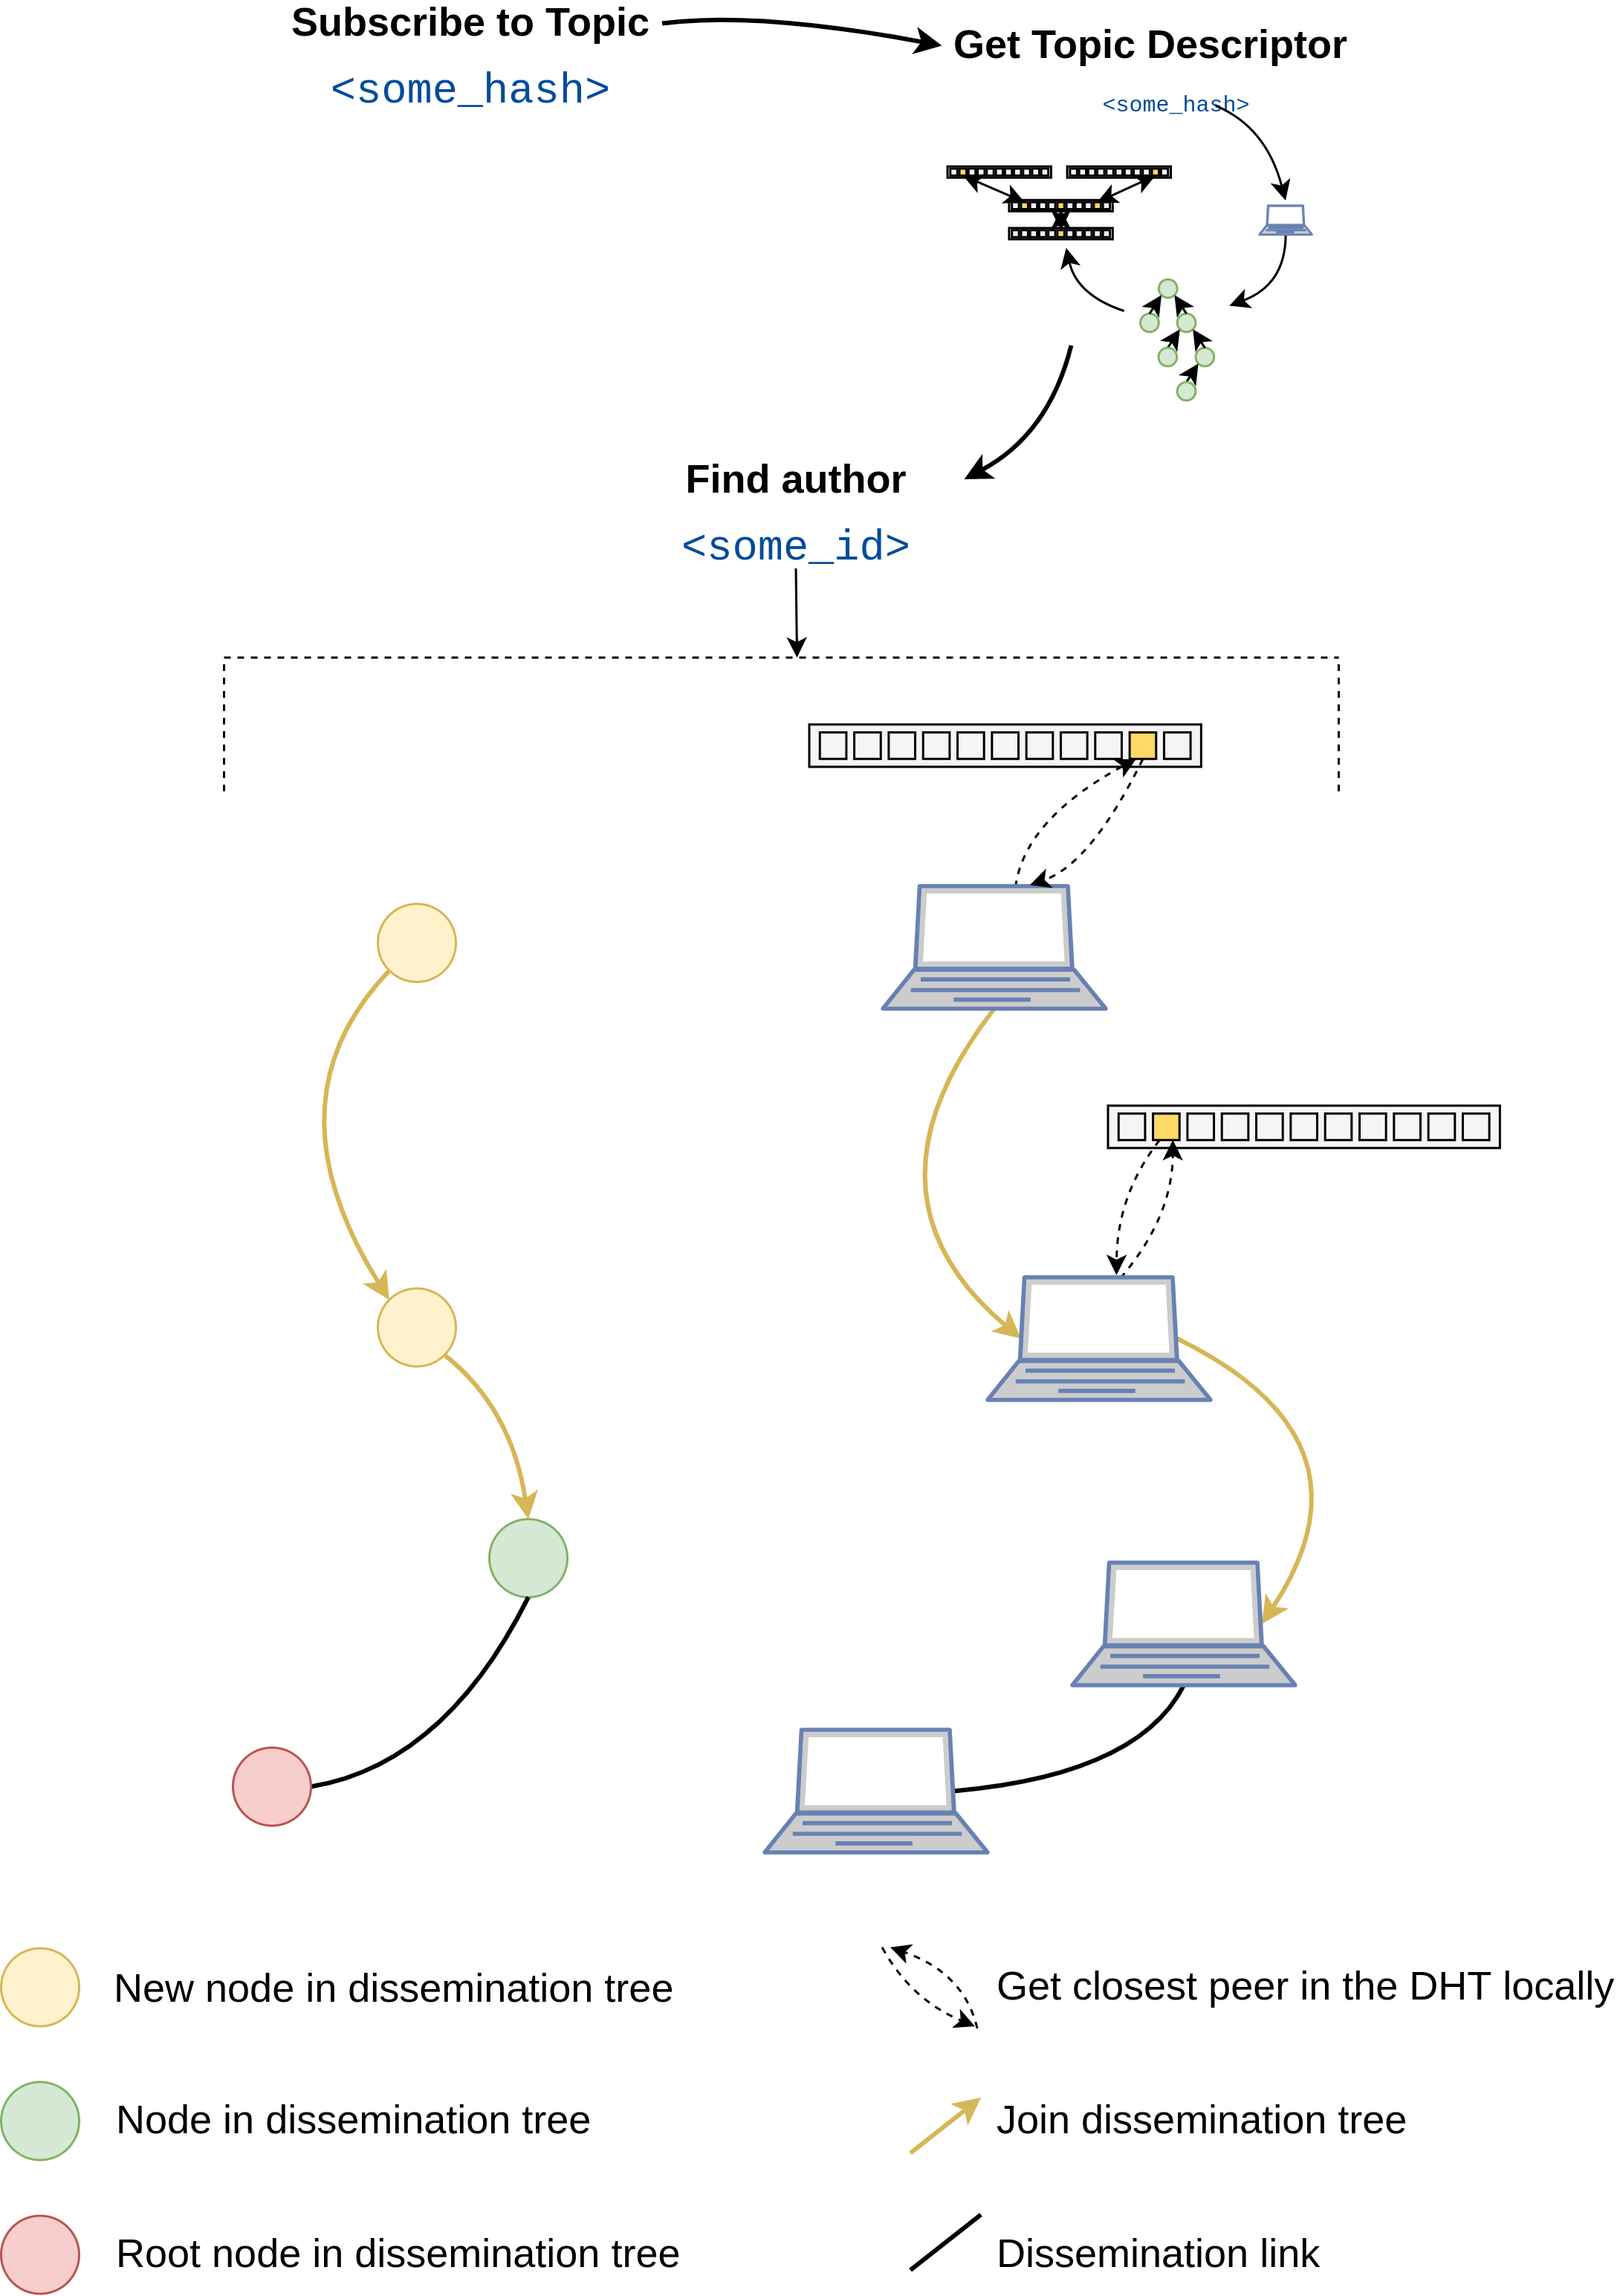
\includegraphics[width=0.4\textwidth]{img/pulsarcast-subscription-flow.png}
  \caption{Overview of the flow for creating a new subscription}
  \label{fig:pulsarcast-subscription-flow}
\end{figure}

Considering the topic creation and subscription management previously discussed
we can see that event dissemination becomes easier to handle, almost as a
consequence of the way the subscription management is built, and dissemination
trees again play their key part here. Pulsarcast, however, allows for some
additional customisation and configuration at the topic level focused on
providing a lot more flexibility to our system. When a node is creating a
topic, it can configure:
\begin{itemize}
  \item
    Which nodes are allowed to publish
  \item
     If and which nodes can request to publish
  \item
    How events are linked together (through the parent link)
\end{itemize}

These options are \emph{requestToPublish}, \emph{allowedPublishers} and
\emph{eventLinking}, all kept under the meta property of the topic descriptor.
Figures \ref{fig:pulsarcast-publish-order-guarantee} and
\ref{fig:pulsarcast-publish-custom} provide visual aids to how these options
come together for event dissemination.

\begin{figure}[hb!]
  \centering
  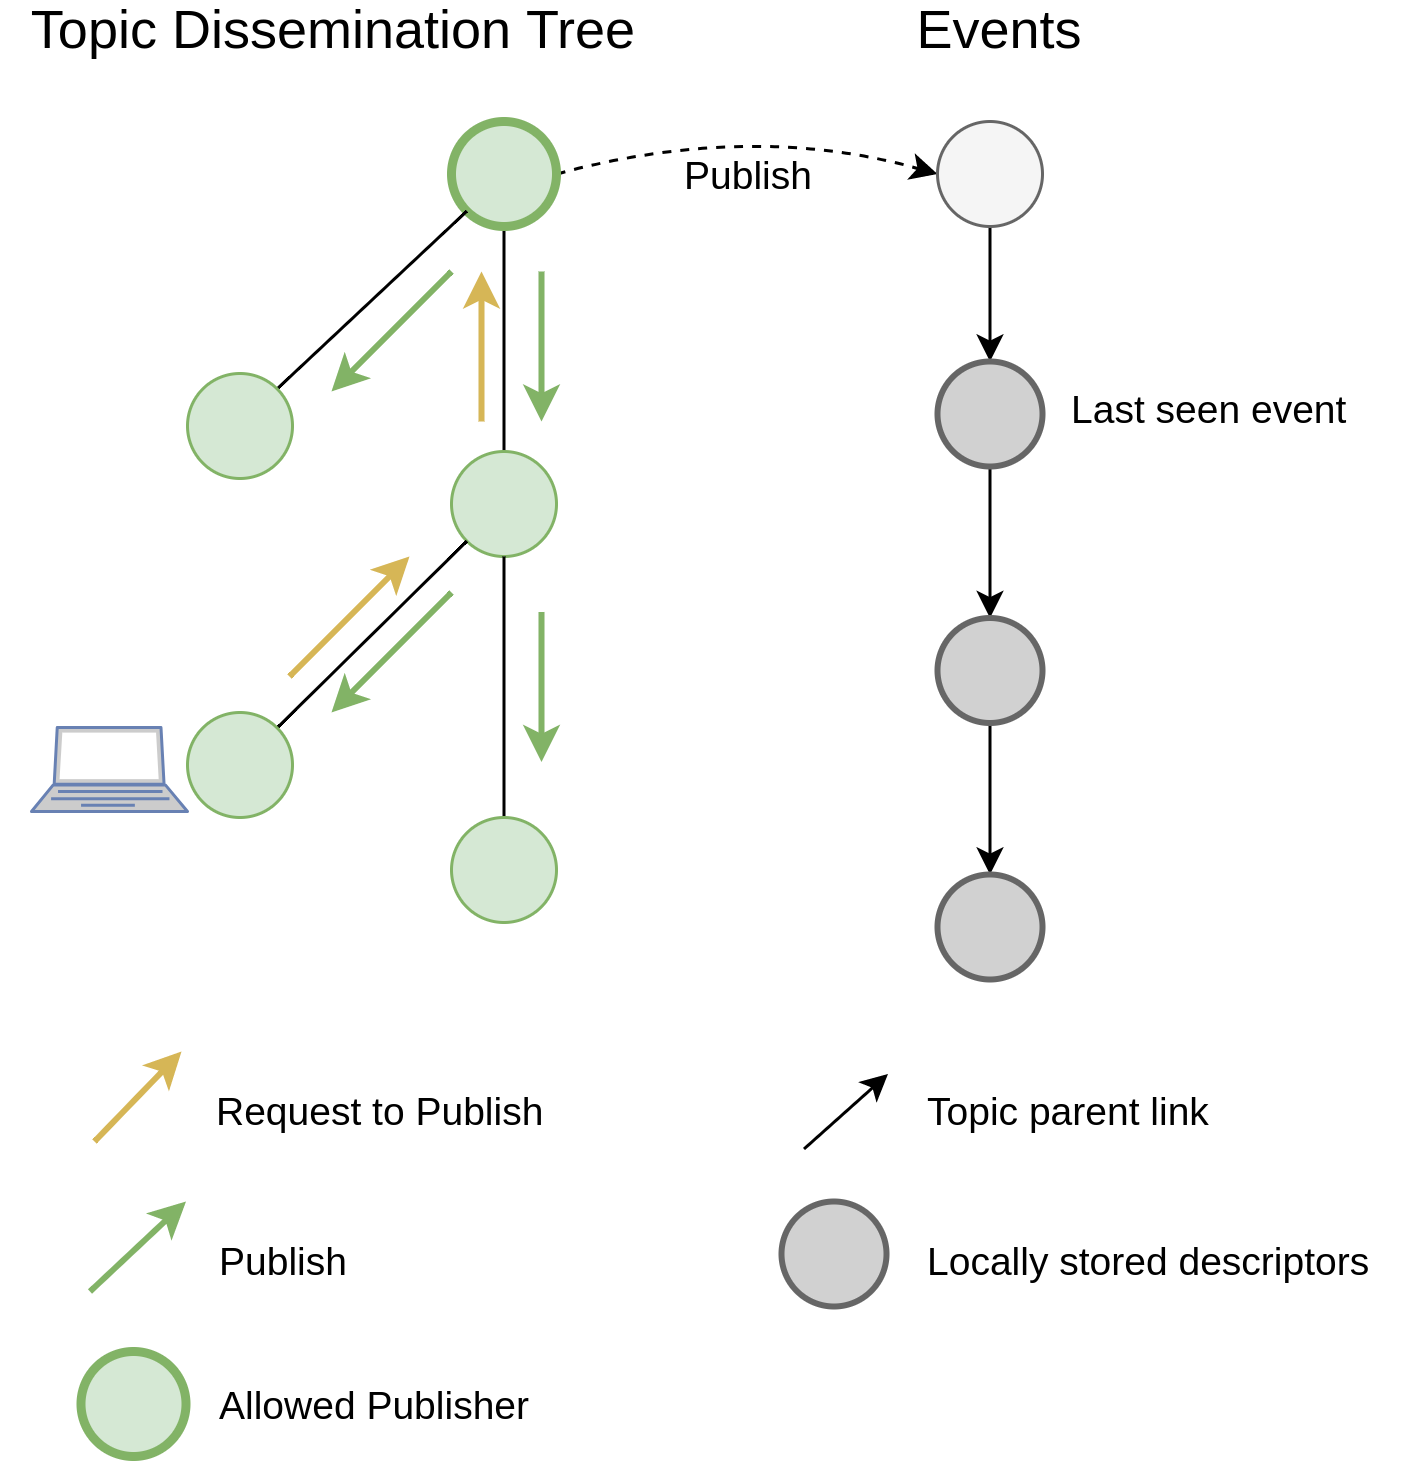
\includegraphics[width=0.3\textwidth]{img/pulsarcast-publish-order-guarantee.png}
  \caption{Event dissemination mechanism for a topic with only the author allowed to publish, last seen event linking and request to publish allowed. This scenario provides order guarantee.}
  \label{fig:pulsarcast-publish-order-guarantee}
\end{figure}

\begin{figure}[hb!]
  \centering
  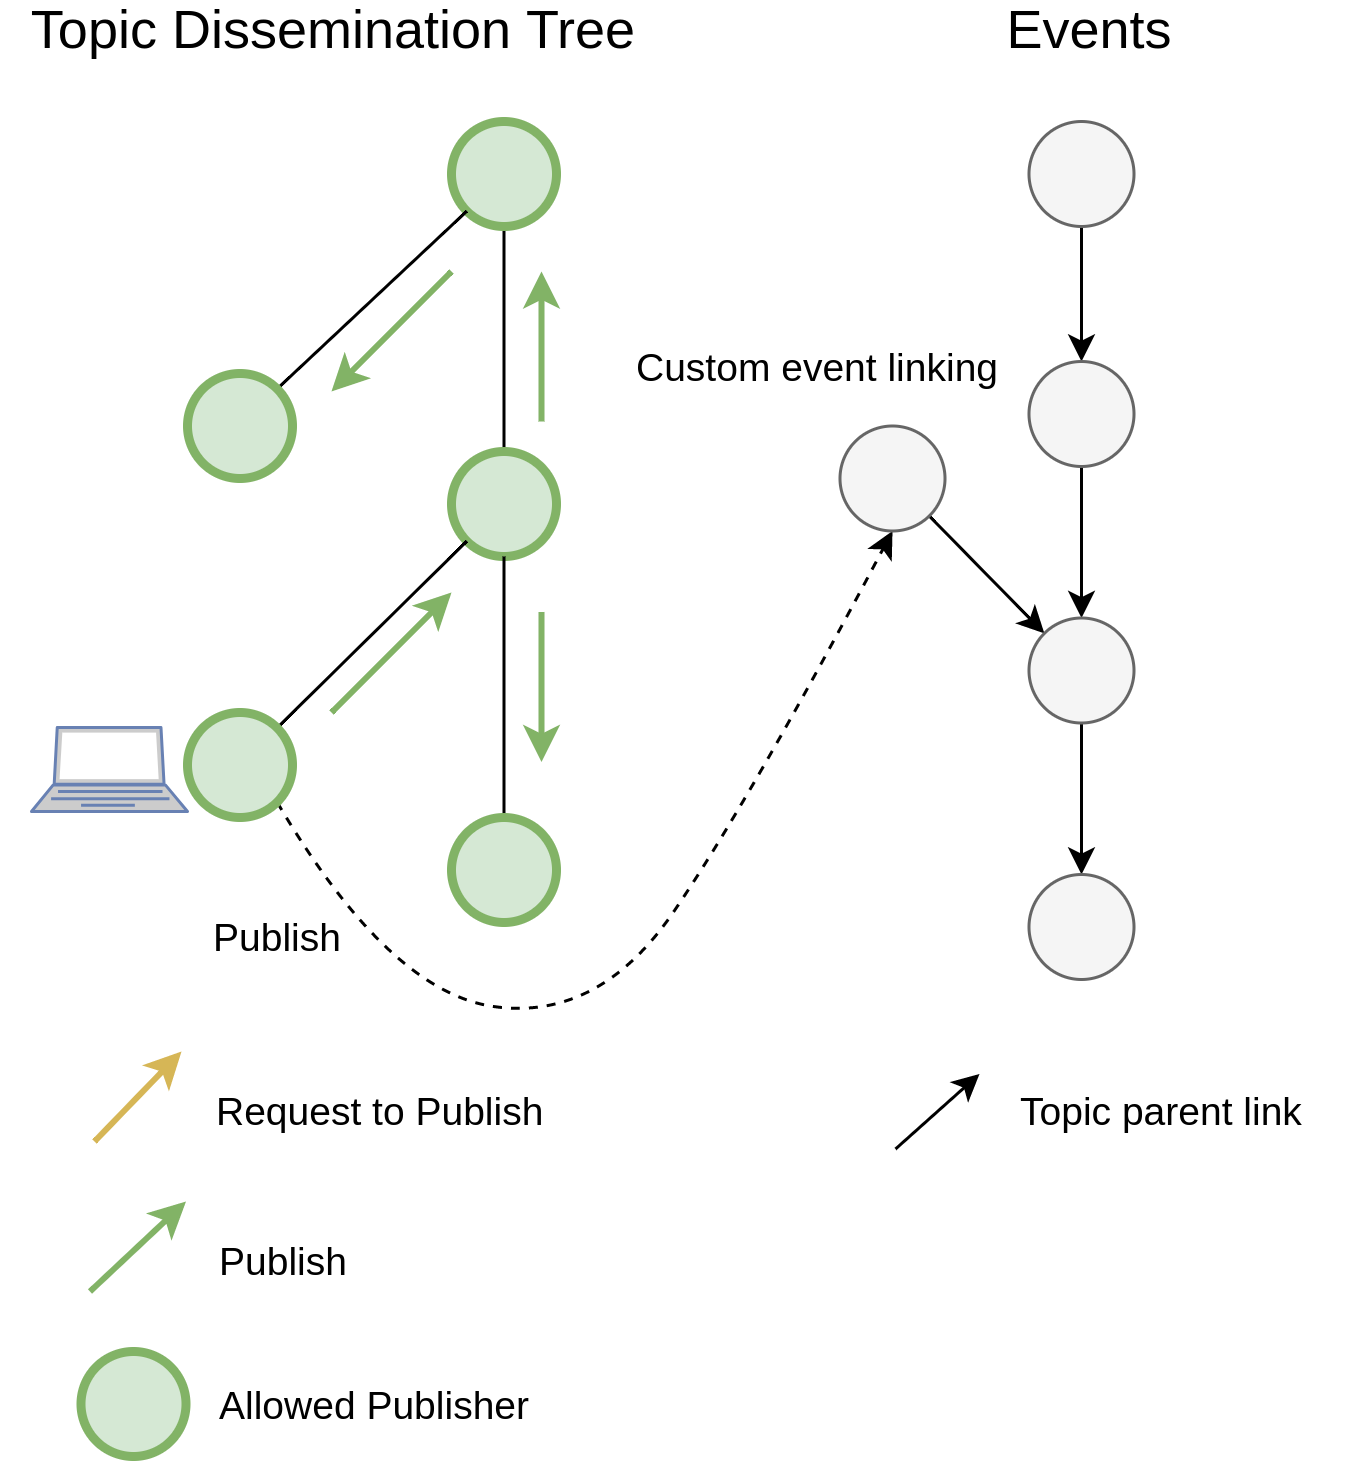
\includegraphics[width=0.3\textwidth]{img/pulsarcast-publish-custom.png}
  \caption{Event dissemination mechanism for a topic with custom event linking and global publishers allowed}
  \label{fig:pulsarcast-publish-custom}
\end{figure}

When a node wants to publish an event in a topic, it starts by fetching the
topic descriptor, first locally and then, if it is not present, from the
Kadmelia DHT. The node then checks if it is allowed to publish through the
topic configuration whitelist mechanism. This option, \emph{allowedPublishers},
can either be enabled and, if so, a list of nodes is provided that is checked
before publishing, or it can be disabled, and in that scenario, every node can
publish a message. If the node cannot publish the message, it will check if it
can submit a request to publish. This request to publish is another option set
in the topic descriptor, through the \emph{requestToPublish} field, that, if
enabled, allows every node in the network to submit these special requests.
Optionally, it can also be a whitelist of nodes allowed to submit these. When a
node forwards a request to publish across the network, it propagates across the
dissemination tree (from children nodes to parents) until it eventually finds a
node which is allowed to publish this event. This will dictate the difference
in the publisher (node who actually publishes the content) and the author (node
responsible for creating the content in the first place).

Upon receiving a publish event request, whether if it was initiated at this
node or through a remote request to publish, the node starts by appropriately
linking the new event to a parent event. This is where the \emph{eventLinking}
option in our topic descriptor comes into play. Right now this option can
either be \emph{CUSTOM} or \emph{LAST\_SEEN}. When the topic allows for custom
linking, the client application can set a custom parent event, as long as it
exists. With the last seen option, however, the Pulsarcast node takes care of
linking the given event to the event last seen by it. After the linking is
done, the node can safely store the event descriptor in the Kademlia DHT,
followed by disseminating it through its children and parent nodes in this
topic dissemination tree. From this point forward, nodes along the
dissemination tree will forward the event across branches of the tree where
this has not gone through. All of the logic we have covered around event
dissemination is better detailed in the Algorithms \ref{alg:receive-event} and
\ref{alg:send-event}.

\begin{algorithm}
  \SetAlgoLined
  \Fn{ReceivedEvent(fromNodeId, eventData)}{
      \KwData{$nodeId=$ node id of this node}
      \KwIn{$fromNodeId=$ sender node id}
      \KwIn{$eventData=$ event descriptor}
        \BlankLine
      \Begin{
        $topicData \leftarrow TopicData(eventData.topicId)$\;
        \eIf{$AllowedToPublish(nodeId, topicData)$}{
                $SendEvent(fromNodeId, eventData)$\;
        }{
                \If{$AllowedToRequestToPublish(nodeId, topicData$}{
                    $SendRequestToPublish(eventData)$\;
                }
            }
      }
    }
  \caption{Event handler for each node}
    \label{alg:receive-event}
\end{algorithm}

\begin{algorithm}
  \SetAlgoLined
  \Fn{SendEvent(eventData)}{
      \KwData{$nodeId=$ node id of this node}
      \KwIn{$fromNodeId=$ sender node id}
      \KwIn{$eventData=$ event descriptor}
        \BlankLine
      \Begin{
        $topicData \leftarrow TopicData(eventData.topicId)$\;
            \If{$IsNewEvent(eventData)$} {
                $linkedEvent \leftarrow LinkEvent(eventData)$\;
                $StoreInDHT(linkedEvent)$\;
            }
            \If{$IsSubscribed(eventData.topicId)$} {
                $EmitEvent(eventData.topicId, eventData)$\;
            }
            \For{$peer \leftarrow Children(eventData.topicId)\ AND$
                $peer \leftarrow Parents(eventData.topicId)$}{
                \If{$fromNodeId \neq peer$}{
                    $SendRPC(eventData, peer)$\;
                }
            }
      }
    }
  \caption{Event forwarding function}
    \label{alg:send-event}
\end{algorithm}

We will now highlight some of the properties these configuration options allow.
The simplest example would be a scenario where only the author of a topic is
allowed to publish, event linking is based on the last seen event and request
to publish is allowed. In this example, despite every node being allowed to
create content, we can achieve order guarantee, with a single stream of events
all linked together. Another example would be a scenario where we have a
whitelist of allowed publishers, no request to publish allowed and last seen
event linking taking place. With this, we get a simple producer/consumer
scenario, with a list of a few selected and vouched for producers that every
node is aware of (that could even be expanded later on by the topic author).
Finally, on the other end of the spectrum, we have a scenario where everyone is
allowed to publish, and custom event linking is allowed. Here, we are
essentially giving the ability for clients and applications to use event trees
to represent data in however they see fit given that, with custom event
linking, applications can shape the event trees however they like. Links can go
as far as to imply event causality if applications are programmed and
configured as such.
